\documentclass[../uwthesis.tex]{subfiles}
 
\begin{document}
\chapter {Introduction}
 
There are many conflicting theories of dyslexia, a learning disorder that specifically affects reading in 5-17\% of the population and cannot be explained by cognitive, sensory, or circumstantial factors \cite{Shaywitz1998Dyslexia.,Snowling2000DyslexiaEdition}. It is broadly (but not universally \cite{Ramus2008WhatDeficit,Pennington2012IndividualModels.}) held that dyslexia that dyslexia is characterized by impaired phonological processing, which includes \textit{understanding that speech can be decomposed into phonemes} and \textit{efficiently manipulating, remembering, and accessing phonemic information} \cite{Wagner1987TheSkills,Snowling1998DyslexiaImplications}. However, it is unclear to what extent the maturation of these skills is a cause or consequence of literacy training or why individuals with dyslexia struggle to master phonological awareness, memory, and automaticity. In a general framework, we might imagine that the first
“disruption” in the phonological processing could occur at one of three stages in the auditory pathway: at the level of extracting relevant information for speech perception from incoming acoustic signals, at the phonemic level (mapping symbols and sounds to discrete phonemes), or at the level of general cognitive processes such as working memory and attention \cite{Serniclaes2004AllophonicDyslexia}. This framework is schematized in Figure~\ref{fig:intro_1}

\begin{figure}
    \centering
    \caption{A schematic of several stages at which phonological processing might by disrupted.}
    \label{fig:intro_1}
    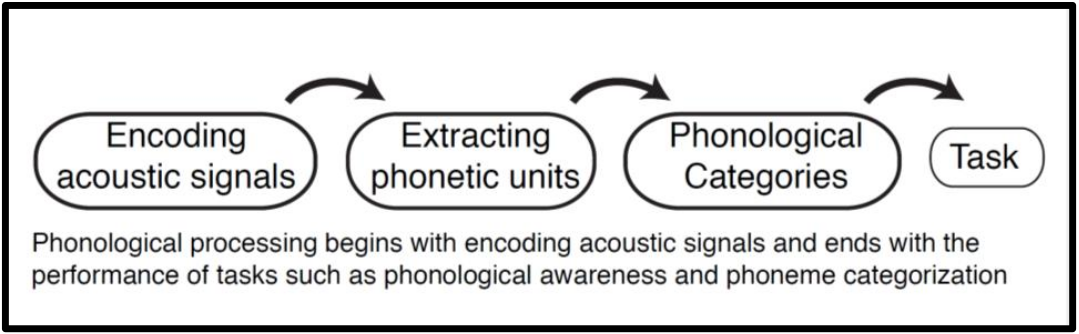
\includegraphics[width=10cm]{images/intro/intro_fig1.png}
\end{figure}
 
In the past decades, several theories have been presented that posit a “core deficit” of dyslexia occurring somewhere in the auditory pathway. Typically, the core deficit is framed as a measurable impairment in some aspect of auditory, linguistic, or cognitive processing that is sufficient to cause dyslexia and accounts for the majority of cases. The purpose of this review is to investigate the evidence supporting the various core deficit theories and to discuss the strengths and weaknesses of these arguments.

It is useful to consider a list of desirable properties that a core deficit model of dyslexia should have:
\begin{itemize}
    \item The deficit must be \textbf{causally related to dyslexia}. An intervention that remedies the deficit in an individual should measurably improve their reading skill.
    \item The deficit must have \textbf{explanatory power as a sensitive and specific mechanism}. In other words, the proposed mechanism should be able to account for the observed impairments in phonological processing, as well as observations from behavioral auditory measures, without simultaneously predicting impairments that individuals with dyslexia do not have.
    \item To be considered a core deficit, the degree of impairment should \textbf{correlate with the degree of reading difficulty}. In other words, in a group of individuals with dyslexia, individuals with the greatest impairment should also have the most disordered reading (in agreement with \cite{Rosen2003AuditoryAnything}).
    \item \textbf{Most individuals with dyslexia should possess the deficit.} Although clinical populations often yield noisy data, we should expect that any impairment warranting the "core deficit" label is broadly applicable. If a deficit does not occur in most individuals with dyslexia, then it should not be framed as the core deficit of dyslexia.
    \item Most individuals with dyslexia should \textbf{fall outside the normal range observed in individuals with typical reading ability}. For example, if individuals with dyslexia perform worse on a given measure but fall overwhelmingly within the 95\% confidence interval of the non-dyslexic population, then that measure likely does not reflect a deficit that in isolation causes dyslexia \cite{Ramus2003TheoriesAdults}. Otherwise, any individual with that deficit would have dyslexia. This pattern may indicate a vulnerability that interacts or adds with other factors to influence reading ability (see Figure~\ref{fig:intro_fig2.png}. But a core deficit should not be present in a substantial proportion of the greater population.
\end{itemize}
 
\begin{figure}
    \centering
    \caption{Simulated distributions of a measure in control and dyslexic groups.}
    \label{fig:intro_fig2.png}
    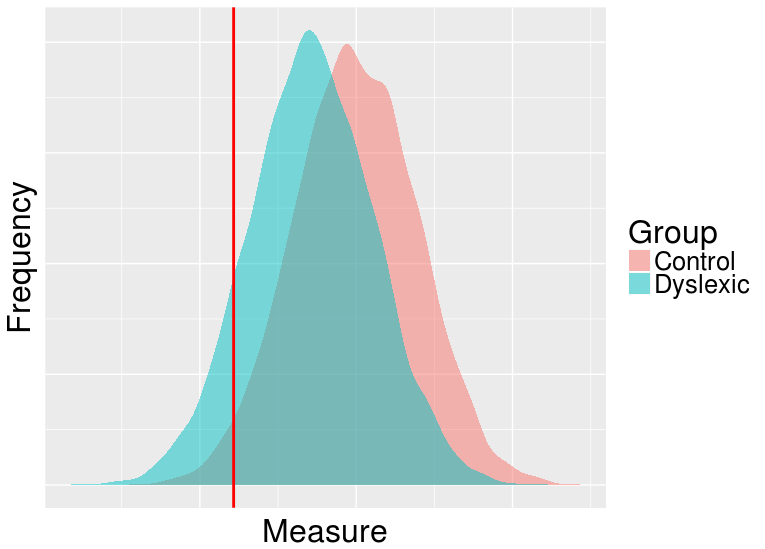
\includegraphics[width=10cm]{images/intro/intro_fig2.png}
    \item \textit{In this example, the
    average value of the measure differs by group, but most measures from the dyslexic group fall within
    the control distribution. The red line indicates the lower bound of the 95\% confidence interval on the
    Control group. Above, an effect size of 0.7 is shown (Cohen’s $d$). This may indicate a risk factor or
    symptom of dyslexia, but implies that in isolation, the process assessed by the measure does not
    cause dyslexia in most individuals.}
\end{figure}

In practice, some of these criteria may be difficult to meet. For example, because a sample of dyslexics is heterogenous in terms of the remedial treatment participants may have received before the study, and because children are unique population with limited capacity for psychophysics, correlations with any measure in a cohort of young dyslexics may be especially noisy. However, we should aspire to hold a high standard of evidence because of the immense effort and financial resources children, families, and teachers will invest in treatments that may appear backed by science.

We begin with a brief review of several prominent theories of dyslexia. Then, we identify several outstanding questions that this dissertation will address. 

\section{Theories of disrputed auditory encoding in dyslexia}

For several decades, sensory deficits in the auditory pathway have been posed to explain poor
phonological awareness in dyslexics. In this framework, compromised neural encoding of acoustic
information leads to poorly specified internal models of phonemes, and consequently “fuzzy”
phonological categories. 

\subsection{The rapid temporal processing hypothesis}
In 1980, Paula Tallal demonstrated that dyslexics as a group performed worse on a temporal
order judgment task with short interstimulus intervals (ISIs) but not long ISIs\cite{Tallal1980AuditoryChildren}. She
concluded that temporal auditory processing is a unique challenge for dyslexics. The proposed
consequence of this alleged deficit would be in processing “rapid” aspects of speech, included formant
transitions and voice onset times. By extension, children would struggle to develop a clear internal
model of the sounds of their language, which would hinder their ability to learn the mappings
between letters and phonemes. This hypothesis was incredibly influential in driving attention to
auditory processing in dyslexics, and the basic tenet—that subtle auditory processing deficits could
jeopardize the development of phonological awareness—still proliferates in many of the auditory
theories of dyslexia that have followed Tallal’s.

Although this hypothesis has been the subject of immense study and discussion for the last
few decades, a great deal of evidence has been aggregated against the conclusion that rapid temporal
processing deficits are at the core of dyslexia. This evidence has previously been summarized (see \cite{Farmer1995TheReview,Rosen2003AuditoryAnything}but is reviewed once again here with inclusion of studies more recently published.

Tallal’s original result, that dyslexics as a group perform worse than controls on temporal
order judgment tasks with brief auditory stimuli, has been replicated. However, four separate studies
have clarified the interpretation of her finding
\cite{Reed1989SpeechChildren,Nittrouer1999DoProblems,Marshall2001RapidDyslexia,Waber2001ProcessingDisorders}.
In Tallal’s original study, most participants were at ceiling performance for the long ISI condition. In the four follow-up studies by other experimenters, creating
conditions where all listeners are below ceiling performance revealed that dyslexics are indeed, on
average, equally deficient performing the task with long ISIs.

There is also abundant evidence that dyslexics are not specifically impaired at processing
brief sounds. In one intensive study where 16 dyslexic adults and 16 controls participated in a battery
of auditory psychophysical tasks, dyslexics as a group performed worse on the auditory measures,
but performance did not differ on tasks that relied on temporal and non-temporal cues \cite{Ramus2003TheoriesAdults}. The same pattern was found in another similarly designed study of dyslexic adults \cite{Amitay2002DisabledDeficit.}. Furthermore, dyslexics as a group seem to be impaired according to several measures of
basic auditory processing that could not be considered “rapid”, including slow (2 Hz) amplitude and
frequency modulation detection 
\cite{Witton1998SensitivityReaders,Lorenzi2000UseDyslexi, Stuart2006ASample}.
Another blow to the notion that briefly presented temporal information is somehow degraded
in dyslexics comes from a recent meta-analysis of basic auditory processing measures showing that
gap detection thresholds are a particularly unreliable predictor of reading ability  \cite{Hamalainen2013BasicDyslexia}. Gap detection thresholds provide evidence that temporal resolution,
the ability to detect brief events in sound, is intact in dyslexics. Clearly, although there are tasks
involving some aspects of temporal processing (such as temporal order judgments) that reveal group
differences, dyslexics are not specifically impaired at these auditory tasks and appear to have normal
temporal resolution.

The reason why we ought to care about rapid temporal processing in dyslexics, in the view of Tallal, is that it creates a specific roadblock for children learning the sounds of their language and mapping them to letters. Children with a “fuzzy” percept of formant transitions---such as those that
differentiate /ba/ from /da/---might in theory struggle to learn how those ambiguous categories relate to discrete letters. 

This idea is inherently problematic for several reasons relating to the nature of the speech signal: first, that temporal cues like formant transitions rarely occur in total isolation
in speech (even /ba/$sim$/da/ contrasts, and VOT contrasts, typically contain spectral cues when
naturally produced). Second, stop consonants are particularly targeted by Tallal’s theory, but “rapid
temporal information” is also part of certain vowels and dipthongs. Accordingly, it is not clear how
an inability to make sense of sound below a temporal resolution of about 40 ms would go entirely
unnoticed in children whose only apparent disability pertains to reading \cite{Nittrouer1999DoProblems}. Indeed,
in a cue-weighting study by Nittrouer et al. (1999), the dyslexic group showed greater weighting of spectrotemporal cues (ie, formant transitions) than spectral cues compared to controls—exactly the opposite of what the rapid temporal processing hypothesis would predict. Furthermore, there is
ample evidence that group differences in speech perception measures (such as phoneme identification and discrimination) occur even when the cues measured are considerably longer than
Tallal’s proposed window \cite{Noordenbos2015TheMeta-Analysis}.

A final note on the temporal processing hypothesis is that the commercially-available intervention created by Tallal and Merzenich, FastForward, appears ungrounded in evidence based
on several failed attempts at replication. While there is no evidence that slowing down speech improves phoneme discriminability for children with dyslexia \cite{Bradlow1999EffectsChildren}, Fast ForWord claims to
rehabilitate struggling readers with exposure to synthetically lengthened speech and training on “rapid auditory processing”. Merzenich and Tallal published promising results claiming that their program improved receptive language skills, although reading skills were not assessed in the original
studies \cite{Merzenich1996TemporalTraining,Tallal1996LanguageSpeech}. Two follow-up studies by Tallal and collaborators addressed reading skill: small samples (20 and 22 dyslexic children) showed significant gains on
standardized reading tests after using the program \cite{Temple2003NeuralMRI,Gaab2007NeuralStudy}.
 
However, these findings are largely at odds with the results found by any other group
employing adequate controls and numbers of participants. There have been several attempts to
assess the efficacy of Fast ForWord by research groups unaffiliated with the program’s creator with
discouraging results. A meta-analysis of six high-quality studies evaluating gains with the Fast
ForWord program in large, individually randomized, controlled trials (60 – 454 participants each)
concluded, “There is no evidence from this review that Fast ForWord is effective as a treatment for
children’s reading or expressive or receptive vocabulary weaknesses” \cite{Strong2011AProgram}. Simply
put, training rapid auditory processing in dyslexic children does not appear to add benefit to
traditional intervention curricula.
 
In sum, there is no longer credible evidence for the hypothesis that dyslexics are specifically impaired at processing brief auditory cues or that such a perceptual deficit plays a causal role in their struggle to acquire fluency in reading. A minority of dyslexics do appear to have abnormal performance on tasks that involve briefly presented cues, but dyslexics appear to have normal temporal resolution as measured by gap detection. There is also ample evidence that group differences in auditory psychophysics are seen in tasks that cannot be considered to involve “rapid” temporal cues. Although reports by the creators of Fast ForWord and their collaborators have
concluded that rapid auditory processing training can improve reading skills, the overwhelming evidence from high-quality, randomized studies by independent investigators does not support this thinking. Thus, rapid temporal processing deficits are unlikely to be a central cause of dyslexia in most cases, and the proposed mechanism is not consistent with the auditory psychophysical literature.

Despite this wealth of evidence against it, the notion that rapid temporal processing difficulties are a hallmark of dyslexia persists in the literature \cite{Vandermosten2010AdultsCues,Vandermosten2011ImpairmentsDifficulties,Goswami2015SensoryResearch}; most recently, this alleged impairment has been cited as evidence for the "neural noise hypothesis" of dyslexia \cite{Hancock}### NEED CITATION###.

\subsection{The slow temporal processing hypothesis}
The “temporal sampling theory” is a relatively recent hypothesis inspired by the temporal sampling framework of audition posed by Poeppel (Poeppel, 2003; Giraud and Poeppel, 2012). In
Poeppel’s model, neural oscillations sample incoming auditory information. Neural oscillations in the 4-10 Hz frequency band (called Theta waves) are thought to be important for coding syllabic information because these endogenous oscillations have been observed to phase lock to syllables in
speech. This process was hypothesized to be disrupted in dyslexics by Goswami \cite{Goswami2011ADyslexia}.

The hypothesis of the temporal sampling framework is that dyslexics abnormally integrate phonetic features with syllabic-rate information, and this somehow leads to irregularly
specified phonemes that are difficult to map to graphemes. The mechanisms of integration across temporal timescales to construct auditory objects are still largely unknown, so the proposed pathway from abnormal entrainment to syllabic-level cues in speech to disordered phonemes remains vague.

However, the theory makes several testable predictions. Although evidence pertaining to neuroimaging and neural recording methods are outside the scope of this review, we can consider predictions that are testable in behavioral paradigms.

The sampling theory predicts in particular that psychophysical measures of rise time processing, as well as amplitude modulation discrimination and detection at low modulation rates, should be impaired in individuals with dyslexia. 





\end{document}